\documentclass[journal,12pt,twocolumn]{IEEEtran}
%
\usepackage{setspace}
\usepackage{gensymb}
\usepackage{xcolor}
\usepackage{caption}
%\usepackage{subcaption}
%\doublespacing
\singlespacing

%\usepackage{graphicx}
%\usepackage{amssymb}
%\usepackage{relsize}
\usepackage[cmex10]{amsmath}
\usepackage{mathtools}
%\usepackage{amsthm}
%\interdisplaylinepenalty=2500
%\savesymbol{iint}
%\usepackage{txfonts}
%\restoresymbol{TXF}{iint}
%\usepackage{wasysym}
\usepackage{hyperref}
\usepackage{amsthm}
\usepackage{mathrsfs}
\usepackage{txfonts}
\usepackage{stfloats}
\usepackage{cite}
\usepackage{cases}
\usepackage{subfig}
%\usepackage{xtab}
\usepackage{longtable}
\usepackage{multirow}
%\usepackage{algorithm}
%\usepackage{algpseudocode}
%\usepackage{enumerate}
\usepackage{enumitem}
\usepackage{mathtools}
%\usepackage{iithtlc}
%\usepackage[framemethod=tikz]{mdframed}
\usepackage{listings}
\usepackage{amsmath}
\usepackage{scalerel}
\setcounter{MaxMatrixCols}{20}

%\usepackage{stmaryrd}


%\usepackage{wasysym}
%\newcounter{MYtempeqncnt}
\DeclareMathOperator*{\Res}{Res}
%\renewcommand{\baselinestretch}{2}
\renewcommand\thesection{\arabic{section}}
\renewcommand\thesubsection{\thesection.\arabic{subsection}}
\renewcommand\thesubsubsection{\thesubsection.\arabic{subsubsection}}

\renewcommand\thesectiondis{\arabic{section}}
\renewcommand\thesubsectiondis{\thesectiondis.\arabic{subsection}}
\renewcommand\thesubsubsectiondis{\thesubsectiondis.\arabic{subsubsection}}

%\renewcommand{\labelenumi}{\textbf{\theenumi}}
%\renewcommand{\theenumi}{P.\arabic{enumi}}

% correct bad hyphenation here
\hyphenation{op-tical net-works semi-conduc-tor}

\lstset{
	language=Python,
	frame=single, 
	breaklines=true,
	columns=fullflexible
}

\newcommand{\longdiv}{\smash{\mkern-0.43mu\vstretch{1.31}{\hstretch{.7}{)}}\mkern-5.2mu\vstretch{1.31}{\hstretch{.7}{)}}}}

\begin{document}
	%
	
	\theoremstyle{definition}
	\newtheorem{theorem}{Theorem}[section]
	\newtheorem{problem}{Problem}
	\newtheorem{proposition}{Proposition}[section]
	\newtheorem{lemma}{Lemma}[section]
	\newtheorem{corollary}[theorem]{Corollary}
	\newtheorem{example}{Example}[section]
	\newtheorem{definition}{Definition}[section]
	%\newtheorem{algorithm}{Algorithm}[section]
	%\newtheorem{cor}{Corollary}
	\newcommand{\BEQA}{\begin{eqnarray}}
		\newcommand{\EEQA}{\end{eqnarray}}
	\newcommand{\define}{\stackrel{\triangle}{=}}
	\newcommand{\myvec}[1]{\ensuremath{\begin{pmatrix}#1\end{pmatrix}}}
	\newcommand{\mydet}[1]{\ensuremath{\begin{vmatrix}#1\end{vmatrix}}}
	\bibliographystyle{IEEEtran}
	%\bibliographystyle{ieeetr}
	
	\providecommand{\nCr}[2]{\,^{#1}C_{#2}} % nCr
	\providecommand{\nPr}[2]{\,^{#1}P_{#2}} % nPr
	\providecommand{\mbf}{\mathbf}
	\providecommand{\pr}[1]{\ensuremath{\Pr\left(#1\right)}}
	\providecommand{\qfunc}[1]{\ensuremath{Q\left(#1\right)}}
	\providecommand{\sbrak}[1]{\ensuremath{{}\left[#1\right]}}
	\providecommand{\lsbrak}[1]{\ensuremath{{}\left[#1\right.}}
	\providecommand{\rsbrak}[1]{\ensuremath{{}\left.#1\right]}}
	\providecommand{\brak}[1]{\ensuremath{\left(#1\right)}}
	\providecommand{\lbrak}[1]{\ensuremath{\left(#1\right.}}
	\providecommand{\rbrak}[1]{\ensuremath{\left.#1\right)}}
	\providecommand{\cbrak}[1]{\ensuremath{\left\{#1\right\}}}
	\providecommand{\lcbrak}[1]{\ensuremath{\left\{#1\right.}}
	\providecommand{\rcbrak}[1]{\ensuremath{\left.#1\right\}}}
	\theoremstyle{remark}
	\newtheorem{rem}{Remark}
	\newcommand{\sgn}{\mathop{\mathrm{sgn}}}
	\providecommand{\abs}[1]{\left\vert#1\right\vert}
	\providecommand{\res}[1]{\Res\displaylimits_{#1}} 
	\providecommand{\norm}[1]{\lVert#1\rVert}
	\providecommand{\mtx}[1]{\mathbf{#1}}
	\providecommand{\mean}[1]{E\left[ #1 \right]}
	\providecommand{\fourier}{\overset{\mathcal{F}}{ \rightleftharpoons}}
	\providecommand{\ztrans}{\overset{\mathcal{Z}}{ \rightleftharpoons}}
	
	%\providecommand{\hilbert}{\overset{\mathcal{H}}{ \rightleftharpoons}}
	\providecommand{\system}{\overset{\mathcal{H}}{ \longleftrightarrow}}
	%\newcommand{\solution}[2]{\textbf{Solution:}{#1}}
	\newcommand{\solution}{\noindent \textbf{Solution: }}
	\providecommand{\dec}[2]{\ensuremath{\overset{#1}{\underset{#2}{\gtrless}}}}
	\numberwithin{equation}{section}
	%\numberwithin{equation}{subsection}
	%\numberwithin{problem}{subsection}
	%\numberwithin{definition}{subsection}
	\makeatletter
	\@addtoreset{figure}{problem}
	\makeatother
	
	\let\StandardTheFigure\thefigure
	%\renewcommand{\thefigure}{\theproblem.\arabic{figure}}
	\renewcommand{\thefigure}{\theproblem}
	
	
	%\numberwithin{figure}{subsection}
	
	\def\putbox#1#2#3{\makebox[0in][l]{\makebox[#1][l]{}\raisebox{\baselineskip}[0in][0in]{\raisebox{#2}[0in][0in]{#3}}}}
	\def\rightbox#1{\makebox[0in][r]{#1}}
	\def\centbox#1{\makebox[0in]{#1}}
	\def\topbox#1{\raisebox{-\baselineskip}[0in][0in]{#1}}
	\def\midbox#1{\raisebox{-0.5\baselineskip}[0in][0in]{#1}}
	
	\vspace{3cm}
	
	\title{ 
		%\logo{
			Digital Signal Processing
			%}
		%	\logo{Octave for Math Computing }
	}
	%\title{
		%	\logo{Matrix Analysis through Octave}{\begin{center}\includegraphics[scale=.24]{tlc}\end{center}}{}{HAMDSP}
		%}
	
	
	% paper title
	% can use linebreaks \\ within to get better formatting as desired
	%\title{Matrix Analysis through Octave}
	%
	%
	% author names and IEEE memberships
	% note positions of commas and nonbreaking spaces ( ~ ) LaTeX will not break
	% a structure at a ~ so this keeps an author's name from being broken across
	% two lines.
	% use \thanks{} to gain access to the first footnote area
	% a separate \thanks must be used for each paragraph as LaTeX2e's \thanks
	% was not built to handle multiple paragraphs
	%
	
	\author{ G V V Sharma$^{*}$ %<-this  stops a space
		\thanks{*The author is with the Department
			of Electrical Engineering, Indian Institute of Technology, Hyderabad
			502285 India e-mail:  gadepall@iith.ac.in.  All content in the manuscript is 
			released under GNU GPL.  Free to use for anything. }% <-this % stops a space
		%\thanks{J. Doe and J. Doe are with Anonymous University.}% <-this % stops a space
		%\thanks{Manuscript received April 19, 2005; revised January 11, 2007.}}
}
% note the % following the last \IEEEmembership and also \thanks - 
% these prevent an unwanted space from occurring between the last author name
% and the end of the author line. i.e., if you had this:
% 
% \author{....lastname \thanks{...} \thanks{...} }
%                     ^------------^------------^----Do not want these spaces!
%
% a space would be appended to the last name and could cause every name on that
% line to be shifted left slightly. This is one of those "LaTeX things". For
% instance, "\textbf{A} \textbf{B}" will typeset as "A B" not "AB". To get
% "AB" then you have to do: "\textbf{A}\textbf{B}"
% \thanks is no different in this regard, so shield the last } of each \thanks
% that ends a line with a % and do not let a space in before the next \thanks.
% Spaces after \IEEEmembership other than the last one are OK (and needed) as
% you are supposed to have spaces between the names. For what it is worth,
% this is a minor point as most people would not even notice if the said evil
% space somehow managed to creep in.



% The paper headers
%\markboth{Journal of \LaTeX\ Class Files,~Vol.~6, No.~1, January~2007}%
%{Shell \MakeLowercase{\textit{et al.}}: Bare Demo of IEEEtran.cls for Journals}
% The only time the second header will appear is for the odd numbered pages
% after the title page when using the twoside option.
% 
% *** Note that you probably will NOT want to include the author's ***
% *** name in the headers of peer review papers.                   ***
% You can use \ifCLASSOPTIONpeerreview for conditional compilation here if
% you desire.




% If you want to put a publisher's ID mark on the page you can do it like
% this:
%\IEEEpubid{0000--0000/00\$00.00~\copyright~2007 IEEE}
% Remember, if you use this you must call \IEEEpubidadjcol in the second
% column for its text to clear the IEEEpubid mark.



% make the title area
\maketitle

%\newpage

\tableofcontents

%\renewcommand{\thefigure}{\thesection.\theenumi}
%\renewcommand{\thetable}{\thesection.\theenumi}

\renewcommand{\thefigure}{\theenumi}
\renewcommand{\thetable}{\theenumi}

%\renewcommand{\theequation}{\thesection}


\bigskip

\begin{abstract}
This manual provides a simple introduction to digital signal processing.
\end{abstract}
\section{Software Installation}
Run the following commands
\begin{lstlisting}
sudo apt-get update
sudo apt-get install libffi-dev libsndfile1 python3-scipy  python3-numpy python3-matplotlib 
sudo pip install cffi pysoundfile 
\end{lstlisting}
\section{Digital Filter}
\begin{enumerate}[label=\thesection.\arabic*
,ref=\thesection.\theenumi]
\item
\label{prob:input}
Download the sound file from  
\begin{lstlisting}
	wget https://raw.githubusercontent.com/gadepall/ 
	EE1310/master/filter/codes/Sound_Noise.wav
\end{lstlisting}
%\href{http://tlc.iith.ac.in/img/sound/Sound_Noise.wav}{\url{http://tlc.iith.ac.in/img/sound/Sound_Noise.wav}}  
%in the link given below.
%\linebreak
\item
\label{prob:spectrogram}
You will find a spectrogram at \href{https://academo.org/demos/spectrum-analyzer}{\url{https://academo.org/demos/spectrum-analyzer}}. 
%\end{problem}
%%
%
%%\onecolumn
%%\input{./figs/fir}
%\begin{problem}
Upload the sound file that you downloaded in Problem \ref{prob:input} in the spectrogram  and play.  Observe the spectrogram. What do you find?
\\
%
\solution There are a lot of yellow lines between 440 Hz to 5.1 KHz.  These represent the synthesizer key tones. Also, the key strokes
are audible along with background noise.
% By observing spectrogram, it clearly shows that tonal frequency is under 4kHz. And above 4kHz only noise is present.
\item
\label{prob:output}
Write the python code for removal of out of band noise and execute the code.
\\
\solution
\lstinputlisting{./codes/Cancel_noise.py}
%\begin{figure}[h]
%\centering
%\includegraphics[width=\columnwidth]{enc_block_diag.png}
%\caption{}
%\label{fig:convolution encoder}
%\end{figure}
%\input{block_enc}
\item
The output of the python script in Problem \ref{prob:output} is the audio file Sound\_With\_ReducedNoise.wav. Play the file in the spectrogram in Problem \ref{prob:spectrogram}. What do you observe?
\\
\solution The key strokes as well as background noise is subdued in the audio.  Also,  the signal is blank for frequencies above 5.1 kHz.

\end{enumerate}
\section{Difference Equation}
\begin{enumerate}[label=\thesection.\arabic*,ref=\thesection.\theenumi]
\item Let
\label{def:xn}
\begin{equation}
	x(n) = \cbrak{\underset{\uparrow}{1},2,3,4,2,1}
\end{equation}
Sketch $x(n)$.
\item Let
\begin{multline}
	\label{eq:iir_filter}
	y(n) + \frac{1}{2}y(n-1) = x(n) + x(n-2), 
	\\
	y(n) = 0, n < 0
\end{multline}
Sketch $y(n)$.  
\\
\solution The following code yields Fig. \ref{fig:xnyn}.
\begin{lstlisting}
	wget https://github.com/gadepall/EE1310/raw/master/filter/codes/xnyn.py
\end{lstlisting}
\begin{figure}[!ht]
	\begin{center}
		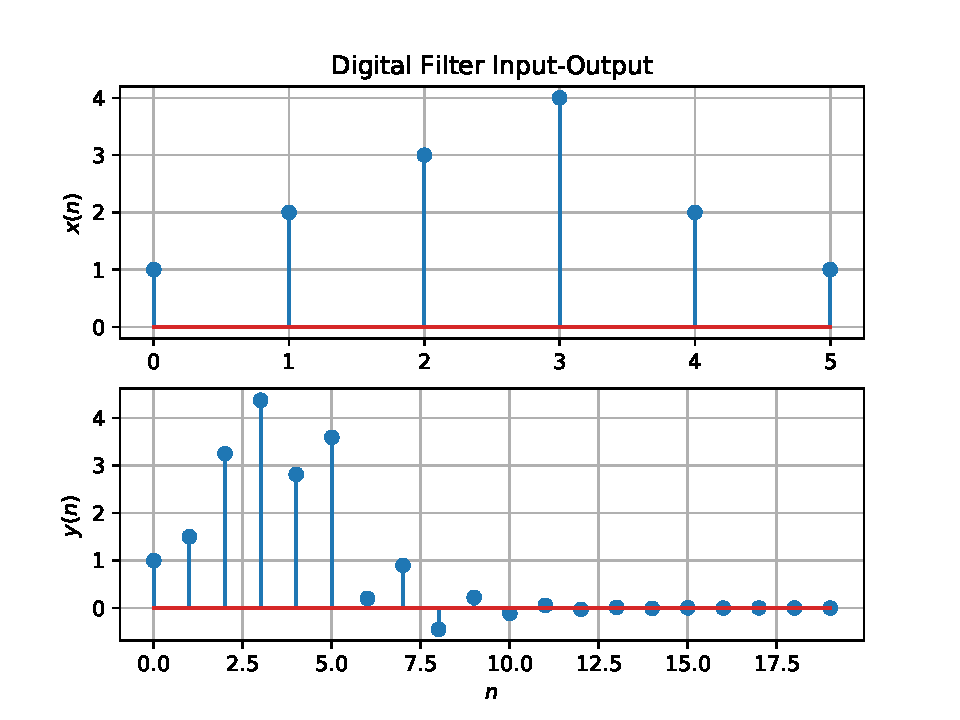
\includegraphics[width=\columnwidth]{./figs/xnyn}
	\end{center}
	\captionof{figure}{}
	\label{fig:xnyn}	
\end{figure}
\item Repeat the above exercise using a C code.
%\\\\\\\\\\\\\\\\\solution
%\lstinputlisting{./codes/xnyn.c}
\end{enumerate}
\section{$Z$-transform}
\begin{enumerate}[label=\thesection.\arabic*]
\item The $Z$-transform of $x(n)$ is defined as
%
\begin{equation}
	\label{eq:z_trans}
	X(z)={\mathcal {Z}}\{x(n)\}=\sum _{n=-\infty }^{\infty }x(n)z^{-n}
\end{equation}
%
Show that
\begin{equation}
	\label{eq:shift1}
	{\mathcal {Z}}\{x(n-1)\} = z^{-1}X(z)
\end{equation}
and find
\begin{equation}
	{\mathcal {Z}}\{x(n-k)\} 
\end{equation}
\solution From \eqref{eq:z_trans},
\begin{align}
	{\mathcal {Z}}\{x(n-k)\} &=\sum _{n=-\infty }^{\infty }x(n-1)z^{-n}
	\\
	&=\sum _{n=-\infty }^{\infty }x(n)z^{-n-1} = z^{-1}\sum _{n=-\infty }^{\infty }x(n)z^{-n}
\end{align}
resulting in \eqref{eq:shift1}. Similarly, it can be shown that
%
\begin{equation}
	\label{eq:z_trans_shift}
	{\mathcal {Z}}\{x(n-k)\} = z^{-k}X(z)
\end{equation}
\item Obtain $X(z)$ for $x(n)$ defined in problem 
\ref{def:xn}.
\solution
From \eqref{eq:z_trans} we get,
\begin{align}
	X(z)&=\sum _{n=-\infty }^{\infty }x(n)z^{-n}\\
	&=x\brak{0}z^{-0} + x\brak{1}z^{-1}+\dots+x\brak{5}z^{-5}\\
	&=1+2z^{-1}+3z^{-2}+4z^{-3}+2z^{-4}+z^{-5}
\end{align}
\item Find
%
\begin{equation}
	H(z) = \frac{Y(z)}{X(z)}
\end{equation}
%
from  \eqref{eq:iir_filter} assuming that the $Z$-transform is a linear operation.
\\
\solution  Applying \eqref{eq:z_trans_shift} in \eqref{eq:iir_filter},
\begin{align}
	Y(z) + \frac{1}{2}z^{-1}Y(z) &= X(z)+z^{-2}X(z)
	\\
	\implies \frac{Y(z)}{X(z)} &= \frac{1 + z^{-2}}{1 + \frac{1}{2}z^{-1}}
	\label{eq:freq_resp}
\end{align}
%
\item Find the Z transform of 
\begin{equation}
	\delta(n)
	=
	\begin{cases}
		1 & n = 0
		\\
		0 & \text{otherwise}
	\end{cases}
\end{equation}
and show that the $Z$-transform of
\begin{equation}
	\label{eq:unit_step}
	u(n)
	=
	\begin{cases}
		1 & n \ge 0
		\\
		0 & \text{otherwise}
	\end{cases}
\end{equation}
is
\begin{equation}
	U(z) = \frac{1}{1-z^{-1}}, \quad \abs{z} > 1
\end{equation}
\solution It is easy to show that
\begin{equation}
	\delta(n) \ztrans 1
\end{equation}
and from \eqref{eq:unit_step},
\begin{align}
	U(z) &= \sum _{n= 0}^{\infty}z^{-n}
	\\
	&=\frac{1}{1-z^{-1}}, \quad \abs{z} > 1
\end{align}
using the fomula for the sum of an infinite geometric progression.
%
\item Show that 
\begin{equation}
	\label{eq:anun}
	a^nu(n) \ztrans \frac{1}{1-az^{-1}} \quad \abs{z} > \abs{a}
\end{equation}
\solution
\begin{align}
	{\mathcal {Z}}\{a^nu(n)\} &= \sum _{n=-\infty }^{\infty }a^nu(n)z^{-n}
	\\&=\sum _{n=0 }^{\infty }a^nz^{-n}
	\\&=\frac{1}{1-az^{-1}}, \quad \abs{z} > \abs{a}
\end{align}
%
\item 
Let
\begin{equation}
	H\brak{e^{\j \omega}} = H\brak{z = e^{\j \omega}}.
\end{equation}
Plot $\abs{H\brak{e^{\j \omega}}}$.  Is it periodic? If so, find the period. $H(e^{\j \omega})$ is
known as the {\em Discret Time Fourier Transform} (DTFT) of $h(n)$.
\\
\solution 
From \eqref{eq:freq_resp} we get
\begin{align}
	H\brak{e^{\j \omega}} &= H\brak{z = e^{\j \omega}}\\
	&=\frac{1 + \brak{e^{-2\j \omega}}}{1 + \frac{1}{2}\brak{e^{-1\j \omega}}}\\
	&=\frac{\brak{e^{\j \omega}} + \brak{e^{-\j \omega}}}{\brak{e^{\j \omega}} + \frac{1}{2}}\\
	&=\frac{2\cos\brak{\omega}}{\brak{e^{\j \omega}} + \frac{1}{2}}\\
	\implies \abs{H\brak{e^{\j \omega}}} &= \frac{2\cos\brak{\omega}}{\sqrt{\brak{\cos\brak{\omega}+\frac{1}{2}}^{2}+\brak{\sin^2\brak{\omega}}}}
\end{align}
\begin{align}
	&=\frac{2\cos\brak{\omega}}{\sqrt{\cos^2\brak{\omega}+\sin^2\brak{\omega}+\cos\brak{\omega}+\frac{1}{4}}}\\
	&=\frac{2\cos\brak{\omega}}{\sqrt{\frac{5}{4}+\cos\brak{\omega}}}\\
\end{align}
For a periodic function of period $T$,
\begin{align}
	f\brak{x} = f\brak{x+T}, T \neq 0	 
\end{align}
Both the numerator and denominator have a period of $2\pi$ since $\cos\brak{\omega}$ has a period of $2\pi$. Which means that $H(e^{\j (\omega)})$ has a period of $2\pi$
%Checking if $2\pi$ is the fundamental period by checking if $\pi$ is also a period,
%\begin{align}
%	\frac{2\cos\brak{\omega+\pi}}{\sqrt{\frac{5}{4}+\cos\brak{\omega+\pi}}} &=
%	\frac{-2\cos\brak{\omega}}{\sqrt{\frac{5}{4}-\cos\brak{\omega}}}\\
%	\implies H\brak{e^{\j \brak{\omega+\pi}}} &\neq H\brak{e^{\j \brak{\omega}}}
%\end{align}
$\therefore$ Period is $2\pi$.\\
The following code plots Fig. \ref{fig:dtft}.
\begin{lstlisting}
	wget https://raw.githubusercontent.com/gadepall/EE1310/master/filter/codes/dtft.py
\end{lstlisting}
\begin{figure}[!ht]
	\centering
	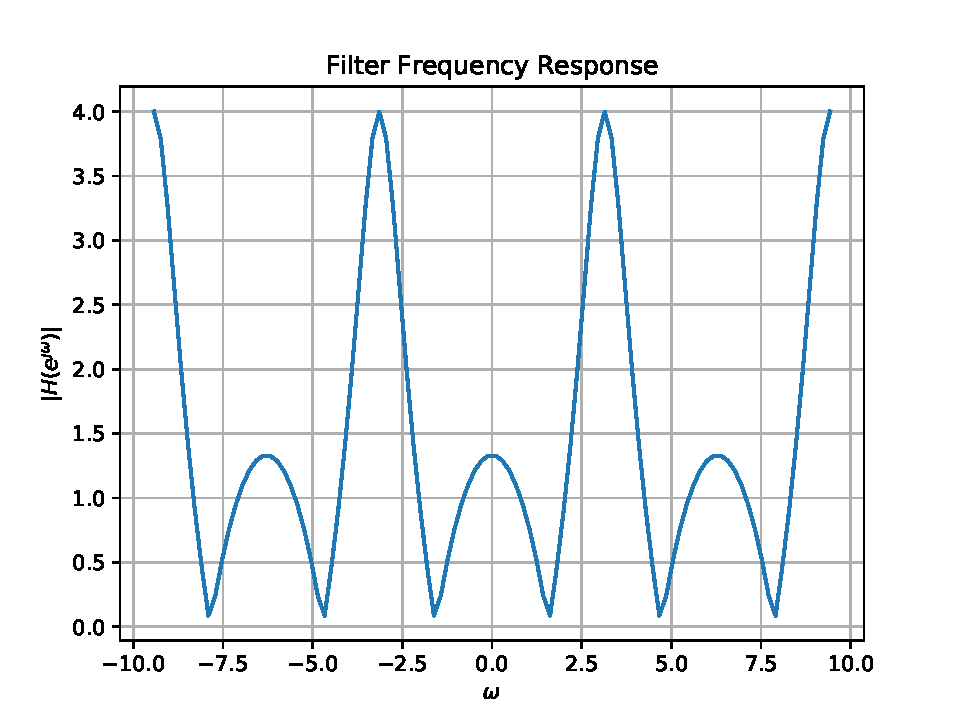
\includegraphics[width=\columnwidth]{./figs/dtft}
	\caption{$\abs{H\brak{e^{\j\omega}}}$}
	\label{fig:dtft}
\end{figure}

From Fig. \ref{fig:dtft} we can see that $\abs{H\brak{e^{\j \omega}}}$ is periodic with period $2\pi$.
\\
\item Express $h(n)$ in terms of $H\brak{e^{\j \omega}}$.\\
\solution
Since $H\brak{e^{\j \omega}}$ is the DTFT of $h\brak{n}$,
\begin{align}
	H\brak{e^{\j \omega}} = \sum _{n=-\infty }^{\infty }h\brak{n}e^{-\j \omega n}
\end{align}
Multiplying both sides with $e^{\j \omega n}$ and integrating we get
\begin{align}
	\int_{-\pi}^{\pi}H\brak{e^{\j \omega}} e^{\j \omega k} d\omega&= \sum _{n=-\infty }^{\infty }h\brak{n}\int_{-\pi}^{\pi}e^{-\j \omega n} e^{\j \omega k}
\end{align}
	Case 1: $n \neq k$
\begin{align}
	\int_{-\pi}^{\pi}H\brak{e^{\j \omega}} e^{\j \omega k} d\omega&= \sum _{n=-\infty }^{\infty }h\brak{n}\int_{-\pi}^{\pi}e^{-\j \omega n} e^{\j \omega k}d\omega \\
	&=\sum _{n=-\infty }^{\infty }h\brak{n}\frac{e^{\j \pi \brak{k-n}}- e^{-\j \pi \brak{k-n}}}{\j \brak{k-n}}\\
	&=0
\end{align}

	Case 2: $n = k$
\begin{align}
	\int_{-\pi}^{\pi}H\brak{e^{\j \omega}} e^{\j \omega k} d\omega&= \sum _{n=-\infty }^{\infty }h\brak{n}\int_{-\pi}^{\pi}e^{-\j \omega n} e^{\j \omega k}d\omega \\
	&=\sum _{n=-\infty }^{\infty }h\brak{n}\int_{-\pi}^{\pi}d\omega \\
	&= 2\pi
\end{align}
\begin{align}
	&\implies \int_{-\pi}^{\pi}H\brak{e^{\j \omega}} e^{\j \omega k} d\omega =2\pi h\brak{n}\\
	&\implies h\brak{n} = \frac{1}{2\pi} \int_{-\pi}^{\pi} H\brak{e^{\j \omega}}e^{\j \omega n} d\omega
\end{align}
\end{enumerate}
\section{Impulse Response}
\begin{enumerate}[label=\thesection.\arabic*]
\item Using long division, 
find
\begin{align}
	h(n), \quad n < 5
\end{align}
for H(z) in 
\eqref{eq:freq_resp}.\\
\solution
From \eqref{eq:freq_resp} we get,
\begin{align}
	H\brak{z} &= \frac{1 + z^{-2}}{1 + \frac{1}{2}z^{-1}}\\
	\implies H\brak{z} &= \frac{1}{1 + \frac{1}{2}z^{-1}} + \frac{z^{-2}}{1 + \frac{1}{2}z^{-1}}\\
	\text{ROC : } \\
	\abs{\frac{z^{-1}}{2}} &\leq 1\\
	\implies \frac{1}{2} &\leq \abs{z}
\end{align}
\begin{align}
	H\brak{z} = \sum_{-\infty}^{\infty} h\brak{n}z^{-n}
\end{align}

\begin{align}
	\frac{1 + z^{-2}}{1 + \frac{1}{2}z^{-1}} &= \sum_{-\infty}^{\infty} h\brak{n}z^{-n}
\end{align}

\[
\arraycolsep=1pt
\renewcommand\arraystretch{1.2}
\begin{array}{*1r @{\hskip\arraycolsep}c@{\hskip\arraycolsep} *{11}r}
	&          & 1 & - & \frac{z^{-1}}{2} & + & \frac{5z^{-2}}{4} & - & \frac{5z^{-3}}{8} & + & \frac{5z^{-4}}{16} & + & \dots  \\
	\cline{2-13}
	1+\frac{z^{-1}}{2} & \longdiv & 1 & + & 0z^{-1} & +  & z^{-2}     & + & 0z^{-3} & + & 0z^{-4} & + & \dots      \\
	&         & 1 & + & \frac{z^{-1}}{2} &  &   &   &      &   &      &   &        \\
	\cline{3-7}
	&          &   &   & \frac{-z^{-1}}{2} & + &  z^{-2} &   &      &   &      &   &        \\
	&          &   &   & \frac{-z^{-1}}{2} & - &  \frac{z^{-1}}{4} &  &   &   &      &   &        \\
	\cline{5-9}
	&          &   &   &   &   & \frac{5z^{-1}}{4} & + &  0z^{-3} &   &      &   &        \\
	&          &   &   &   &   & \frac{5z^{-1}}{4} & + & \frac{5z^{-3}}{8} &  &  &   &        \\
	\cline{7-11}
	&          &   &   &   &   &      &   & \frac{-5z^{-3}}{8} & + & 0z^{-4} &   &        \\
	&          &   &   &   &   &      &   & \frac{-5z^{-3}}{8} & - & \frac{5z^{-4}}{16} &  &    \\
	\cline{9-13}
	&          &   &   &   &   &      &   &      &   & \frac{5z^{-4}}{16} & + & 0z^{-5}   \\
	&          &   &   &   &   &      &   &      &   &      &   & \vdots \\
\end{array}
\]
Comparing coefficients of $z^{-n}$ we get,
\begin{align}
	h(n) = \begin{cases}
		0 \quad &\text{if}\, n<0\\
		1 \quad &\text{if}\, n=0\\
		\frac{-1}{2} \quad &\text{if}\, n=1\\
		\frac{5}{4} \quad &\text{if}\, n=2\\
		\frac{-5}{8} \quad &\text{if}\, n=3\\
		\frac{5}{16} \quad &\text{if}\, n=4\\
	\end{cases}
\end{align}
		\item \label{prob:impulse_resp}
Find an expression for $h(n)$ using $H(z)$, given that 
%in Problem \ref{eq:ztransab} and \eqref{eq:anun}, given that
\begin{equation}
	\label{eq:impulse_resp}
	h(n) \ztrans H(z)
\end{equation}
and there is a one to one relationship between $h(n)$ and $H(z)$. $h(n)$ is known as the {\em impulse response} of the
system defined by \eqref{eq:iir_filter}.
\\
\solution From \eqref{eq:freq_resp},
\begin{align}
	H(z) &= \frac{1}{1 + \frac{1}{2}z^{-1}} + \frac{ z^{-2}}{1 + \frac{1}{2}z^{-1}}
	\\
	\therefore h(n) &= \brak{-\frac{1}{2}}^{n}u(n) + \brak{-\frac{1}{2}}^{n-2}u(n-2)
\end{align}
using \eqref{eq:anun} and \eqref{eq:z_trans_shift}.
\item Sketch $h(n)$. Is it bounded? Justify theoretically.
\\
\solution 
\begin{align}
	&\abs{u\brak{n}}\leq 1\\
	&\abs{\brak{\frac{-1}{2}}^n}\leq 1\\
	\implies &\abs{\brak{\frac{-1}{2}}^n u\brak{n}}\leq 1\\
	&\text{Similarly,}\\
	\implies &\abs{\brak{\frac{-1}{2}}^{n-2} u\brak{n-2}}\leq 1\\
	\implies &\abs{\brak{\frac{-1}{2}}^n u\brak{n}}+\abs{\brak{\frac{-1}{2}}^{n-2} u\brak{n-2}} \leq 2\\
	\implies &\abs{\brak{\frac{-1}{2}}^n u\brak{n}+\brak{\frac{-1}{2}}^{n-2} u\brak{n-2}}\leq 2
\end{align} 


The following code plots Fig. \ref{fig:hn}.
\begin{lstlisting}
	wget https://raw.githubusercontent.com/gadepall/EE1310/master/filter/codes/hn.py
\end{lstlisting}
\begin{figure}[!ht]
	\centering
	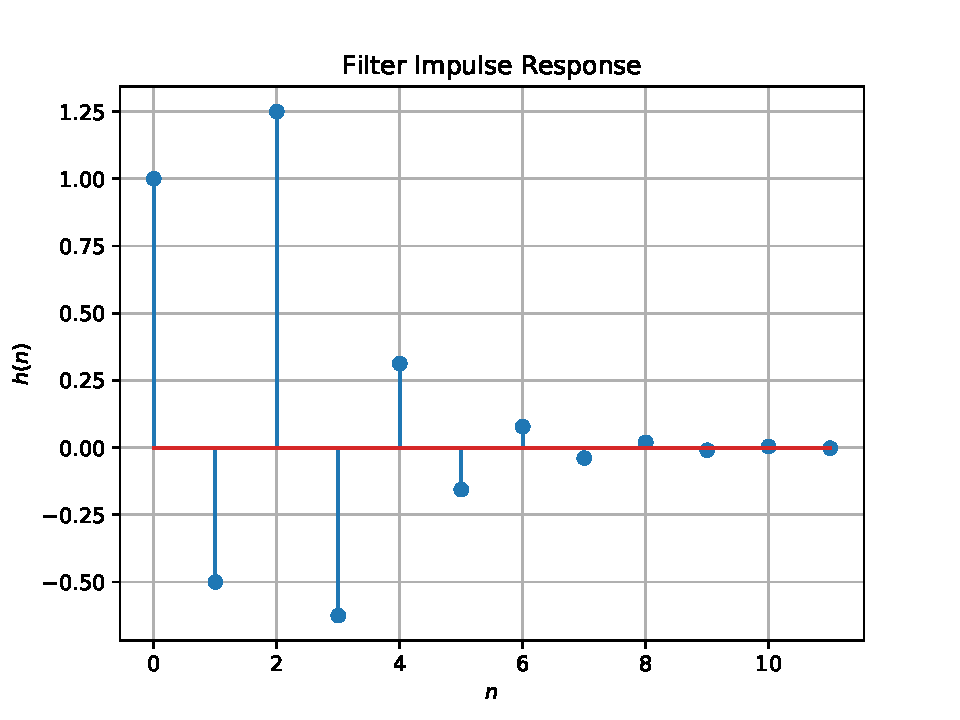
\includegraphics[width=0.9\columnwidth]{./figs/hn}
	\caption{$h(n)$ as the inverse of $H(z)$}
	\label{fig:hn}
\end{figure}
%	\vspace{7.5cm}
\item Convergent? Justify using the ratio test.\\
\solution\\
\begin{align}
	\onehalfspacing
	h(n) = \begin{cases}
		\doublespacing
		0 \quad $if \quad$ n < 0\\
		1, \quad $if \quad$ n = 0\\
		-\frac{1}{2}$, \quad if \quad$ n = 1\\
		5\brak{-\tfrac{1}{2}}^{n}$, \quad if \quad$ n \ge 2
	\end{cases}\\
	\intertext{Using ratio test:}
	\lim_{n \rightarrow \infty} \abs{\dfrac{h(n+1)}{h(n)}} = \abs{\dfrac{5\brak{-\tfrac{1}{2}}^{n+1}}{5\brak{-\tfrac{1}{2}}^{n}}}
	= \frac{1}{2} < \infty
\end{align}
\singlespacing
$\implies h(n)$ is convergent\\
\item The system with $h(n)$ is defined to be stable if
\begin{equation}
	\sum_{n=-\infty}^{\infty}h(n) < \infty
\end{equation}
Is the system defined by \eqref{eq:iir_filter} stable for the impulse response in \eqref{eq:impulse_resp}\\
\solution
\begin{align}
	\sum_{n=-\infty}^{\infty}h(n) = 0 + 1 - \frac{1}{2} + 5\sum_{n=2}^{\infty} \brak{-\dfrac{1}{2}}^{n}\\
	= \dfrac{1}{2} + 5\brak{1 - \dfrac{1}{2} - \brak{\dfrac{1}{1 + \tfrac{1}{2}}}}\\
	= \dfrac{1}{2} + \dfrac{5}{6} = \dfrac{8}{6} = 1.333 < \infty
\end{align}
$\therefore h(n)$  is Stable\\
\item Verify the above result using a python code.\\
\solution The Following code computes and proves the aboves result
\begin{lstlisting}
	wget https://github.com/DarkWake9/EE3900/blob/main/Assignment%201/e5-6.py
\end{lstlisting}
\item 
Compute and sketch $h(n)$ using 
\begin{equation}
	\label{eq:iir_filter_h}
	h(n) + \frac{1}{2}h(n-1) = \delta(n) + \delta(n-2), 
\end{equation}
%
This is the definition of $h(n)$.
\\\\
\solution The following code plots Fig. \ref{fig:hndef}. Note that this is the same as Fig. \ref{fig:hn}. \\\\
\begin{lstlisting}
	wget https://raw.githubusercontent.com/gadepall/EE1310/master/filter/codes/hndef.py
\end{lstlisting}
\begin{figure}[!ht]
	\centering
	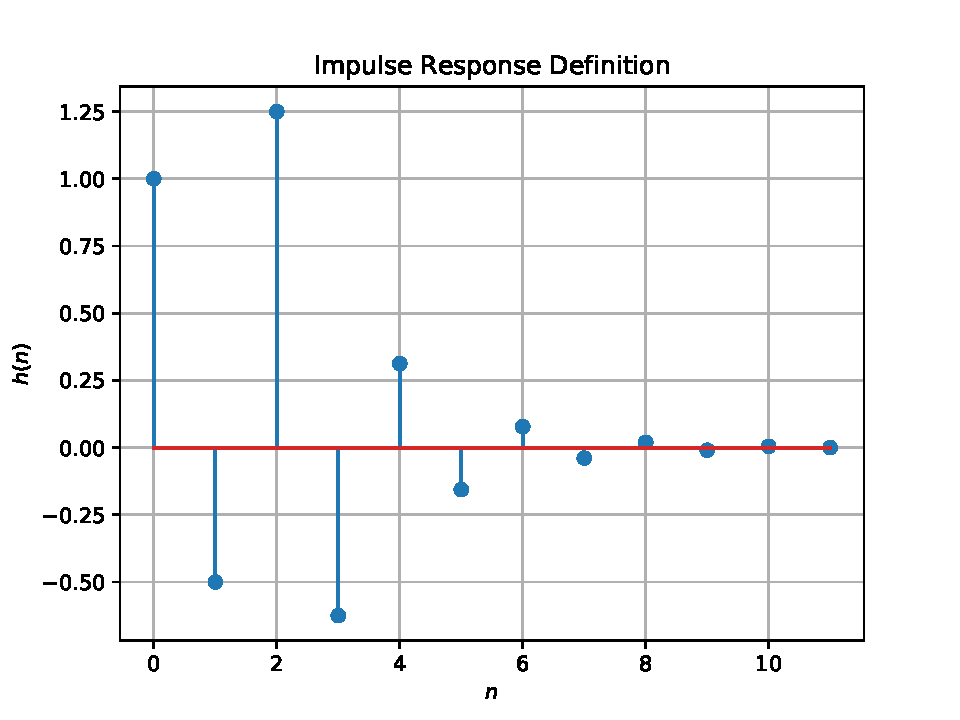
\includegraphics[width=\columnwidth]{./figs/hndef}
	\caption{$h(n)$ from the definition}
	\label{fig:hndef}
\end{figure}
%		\\[100pt]
\item Compute 
%
\begin{equation}
	\label{eq:convolution}
	y(n) = x(n)*h(n) = \sum_{n=-\infty}^{\infty}x(k)h(n-k)
\end{equation}

Comment. The operation in \eqref{eq:convolution} is known as
{\em convolution}.

\solution The following code plots Fig. \ref{fig:ynconv}. Note that this is the same as 
$y(n)$ in  Fig. 
\ref{fig:xnyn}. 
%
\begin{lstlisting}
	wget https://raw.githubusercontent.com/gadepall/EE1310/master/filter/codes/ynconv.py
\end{lstlisting}
\begin{figure}[!ht]
	\centering
	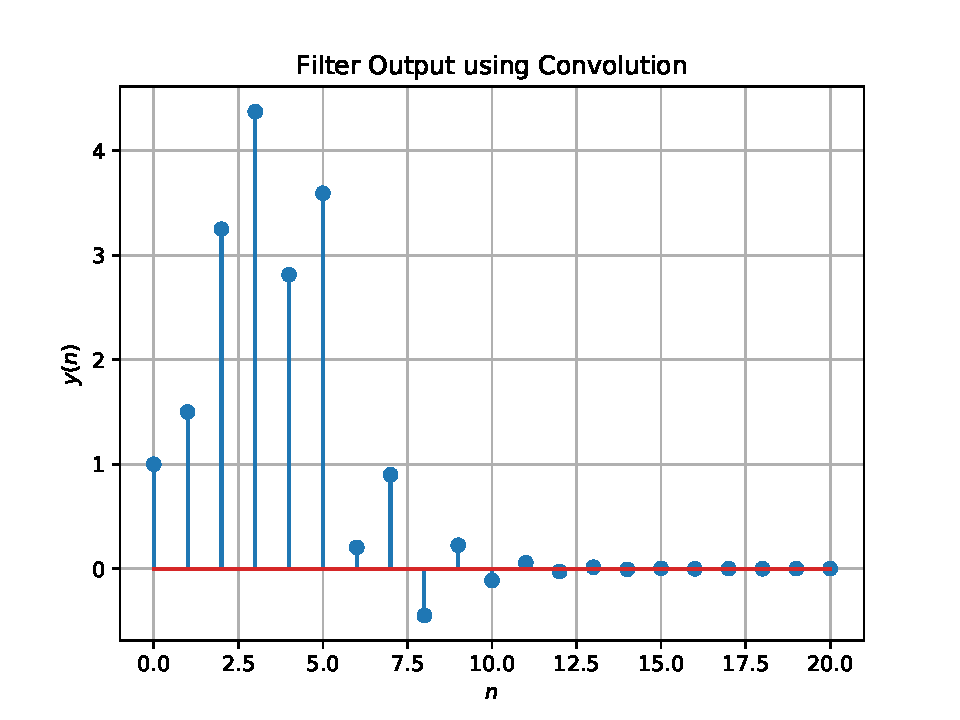
\includegraphics[width=\columnwidth]{./figs/ynconv}
	\caption{\small $y(n)$ from the definition of convolution}
	\label{fig:ynconv}
\end{figure}
\vspace{5cm}
\item Express the above convolution using a Teoplitz matrix.\\
\solution From \eqref{def:xn}
$x(n) = \cbrak{1,2,3,4,2,1}$\\
From \eqref{eq:convolution}	$y(n) = x(n)*h(n)$\\
%			n = 0, $\ldots$ 6\\
\begin{equation}
	\scriptsize 
	\left(
	\begin{smallmatrix}
		x(1) & 0 & 0 & 0 & 0 & 0 & 0 & 0 & 0 & 0 & 0 & 0\\
		x(2) & x(1) & 0 &0 & 0 & 0 & 0 & 0 &  0 & 0 & 0 & 0\\
		x(3) & x(2) & x(1) & 0 & 0 & 0 & 0 &  0 & 0 & 0 & 0 & 0\\
		x(4) & x(3) & x(2) & x(1) & 0 & 0 & 0 & 0 & 0 & 0 & 0 & 0\\
		x(5) & x(4) & x(3) & x(2)&x(1) & 0 & 0 & 0 & 0 & 0 & 0 & 0\\
		x(6) & x(5) & x(4) & x(3)&x(2)&x(1)&0&0&0&0&0&0\\
		0 & x(6) & x(5) & x(4)&x(3)&x(2)&x(1)&0&0&0&0&0\\
		0 & 0 & x(6) & x(5)& x(4)&x(3)&x(2)&x(1)&0&0&0&0\\
		0 & 0 & 0 & x(6) & x(5)&x(4)&x(3)&x(2)&x(1)&0&0&0\\
		0 & 0 & 0 & 0 & x(6) & x(5)&x(4)&x(3)&x(2)&x(1)&0&0\\
		0 & 0 & 0 & 0 & 0 & x(6)&x(5)&x(4)&x(3)&x(2)&x(1)&0\\
		0 & 0 & 0 & 0 & 0 & 0 &x(6)&x(5)&x(4)&x(3)&x(2)&x(1)\\
		0 & 0 & 0 & 0 & 0 & 0 & 0 & x(6)&x(5)&x(4)&x(3)&x(2)\\
		0 & 0 & 0 & 0 & 0 & 0 & 0 & 0 &x(6)&x(5)&x(4)&x(3)\\
		0 & 0 & 0 & 0 & 0 & 0 & 0 & 0 & 0 &x(6)&x(5)&x(4)\\
		0 & 0 & 0 & 0 & 0 & 0 & 0 & 0 & 0 & 0 &x(6)&x(5)\\
		0 & 0 & 0 & 0 & 0 & 0 & 0 & 0 & 0 & 0 & 0 &x(6)\\
		0 & 0 & 0 & 0 & 0 & 0 & 0 & 0 & 0 & 0 & 0 & 0\\
	\end{smallmatrix}
	\right)
	\left(
	\begin{smallmatrix}
		h(1)\\h(2)\\h(3)\\h(4)\\h(5)\\h(6)\\h(7)\\h(8)\\h(9)\\h(10)\\h(11)\\h(12)
	\end{smallmatrix}
	\right)	
	\normalsize
\end{equation}	
\begin{align}
	\left(	\begin{smallmatrix}
		1&0&0&0&0&0&0&0&0&0&0&0\\
		2&1&0&0&0&0&0&0&0&0&0&0\\
		3&2&1&0&0&0&0&0&0&0&0&0\\
		4&3&2&1&0&0&0&0&0&0&0&0\\
		2&4&3&2&1&0&0&0&0&0&0&0\\
		1&2&4&3&2&1&0&0&0&0&0&0\\
		0&1&2&4&3&2&1&0&0&0&0&0\\
		0&0&1&2&4&3&2&1&0&0&0&0\\
		0&0&0&1&2&4&3&2&1&0&0&0\\
		0&0&0&0&1&2&4&3&2&1&0&0\\
		0&0&0&0&0&1&2&4&3&2&1&0\\
		0&0&0&0&0&0&1&2&4&3&2&1\\
		0&0&0&0&0&0&0&1&2&4&3&2\\
		0&0&0&0&0&0&0&0&1&2&4&3\\
		0&0&0&0&0&0&0&0&0&1&2&4\\
		0&0&0&0&0&0&0&0&0&0&1&2\\
		0&0&0&0&0&0&0&0&0&0&0&1\\
		0&0&0&0&0&0&0&0&0&0&0&0\\
	\end{smallmatrix} \right)
	\left(\begin{smallmatrix}1.   \\      -0.5    \\     1.25   \\    -0.625   \\    0.3125  \\   -0.15625 \\ 0.078125  \\  -0.0390625 \\  0.01953125 \\ -0.00976562 \\ 0.00390625 \\ -0.00195312
	\end{smallmatrix} \right)\\
	= \left(\begin{smallmatrix}
		1 \\ 1.5 \\ 3.25\\ 4.375\\
		2.8125 \\ 3.59375 \\ 0.203125 \\ 0.8984375\\
		-0.44921875 \\ 0.224609375 \\-0.112304688 \\ 0.0561523438\\
		-0.0280761719 \\ 0.0140380859 \\-7.01904297  \times 10^{-3} \\ 3.50952148 \times 10^{-3}\\
		-1.75476074 \times 10^{-3} \\ 8.77380371  \times 10^{-4} \\-4.38690186 \times 10^{-4} \\\\ 0 \\\\
	\end{smallmatrix}\right)
\end{align}		
\item Show that
\begin{equation}
	y(n) =  \sum_{n=-\infty}^{\infty}x(n-k)h(k)
\end{equation}
\solution
\begin{align}
	X(z) = {\mathcal{Z}} \{x(n)\}=\sum_{n=-\infty}^{\infty} x(n) z^{-n} \\
	H(z) = {\mathcal{Z}} \{h(m)\}=\sum_{m=-\infty}^{\infty} h(m) z^{-m} \\
	Y(z) = {\mathcal{Z}} \{h(m)\}=\sum_{k=-\infty}^{\infty} y(m) z^{-k}
\end{align}

\begin{align}
	X(z)H(z)=\sum_{n=-\infty}^{\infty} x(n) z^{-n} \sum_{m=-\infty}^{\infty} h(m) z^{-m}\\
	=\sum_{n=-\infty}^{\infty} \sum_{m=-\infty}^{\infty} x[n] h[m] z^{-(n+m)} \\
	\intertext{Let $m = k - n$}
	=\sum_{k=-\infty}^{\infty}\brak{\sum_{n=-\infty}^{\infty} x[n] h[n-k]} z^{-k} \\
	=\sum_{k=-\infty}^{\infty} y[n] z^{-k}=Y($z$) \\
	\implies Y(z) = X(z) \cdot H(z)
\end{align}

now put $n+m=k \quad n=-\infty$

\begin{align}
	\Rightarrow Y(z)=\sum_{k=-\infty}^{\infty} x(m-k) \sum_{m=-\infty}^{\infty} h(m) z^{-k} \\
	=\sum_{k=-\infty}^{\infty}\left(\sum_{m=-\infty}^{\infty} x[m-k] h[k]\right) z^{-k} \\
	\text { but } Y(z)=\sum_{k=-\infty}^{\infty} y(m) z^{-k} \\
	\Rightarrow y(m)=\sum_{m=-\infty}^{\infty} x[m-k] h(k) \\
	\implies y(n)=\sum_{n=-\infty}^{\infty} x(n-k) h(k) 
\end{align}

\end{enumerate}

\section{DFT}
\begin{enumerate}[label=\thesection.\arabic*]
	\item
	Compute
	\begin{equation}
		X(k) \define \sum _{n=0}^{N-1}x(n) e^{-\j2\pi kn/N}, \quad k = 0,1,\dots, N-1
	\end{equation}
	and $H(k)$ using $h(n)$.
	\item Compute 
	\begin{equation}
		Y(k) = X(k)H(k)
		\label{eq:fp}
	\end{equation}
	\item Compute
	\begin{equation}
		y\brak{n}={\frac {1}{N}}\sum _{k=0}^{N-1}Y\brak{k}\cdot e^{\j 2\pi kn/N},\quad n = 0,1,\dots, N-1
		\label{eq:inv-ft}
	\end{equation}
	\solution The following code plots Fig. \eqref{fig:y-n-dft} and computes $X(k)$
	and $Y(k)$. Note that this is the same as $y(n)$ in Fig. \eqref{fig:xnyn}.
	\begin{lstlisting}
		$ wget https://raw.githubusercontent.com/prajwal-3-14159/EE3900_ma20btech11013/main/filter/codes/problem_6-3.py
	\end{lstlisting}
	\begin{figure}[!ht]
		\centering
		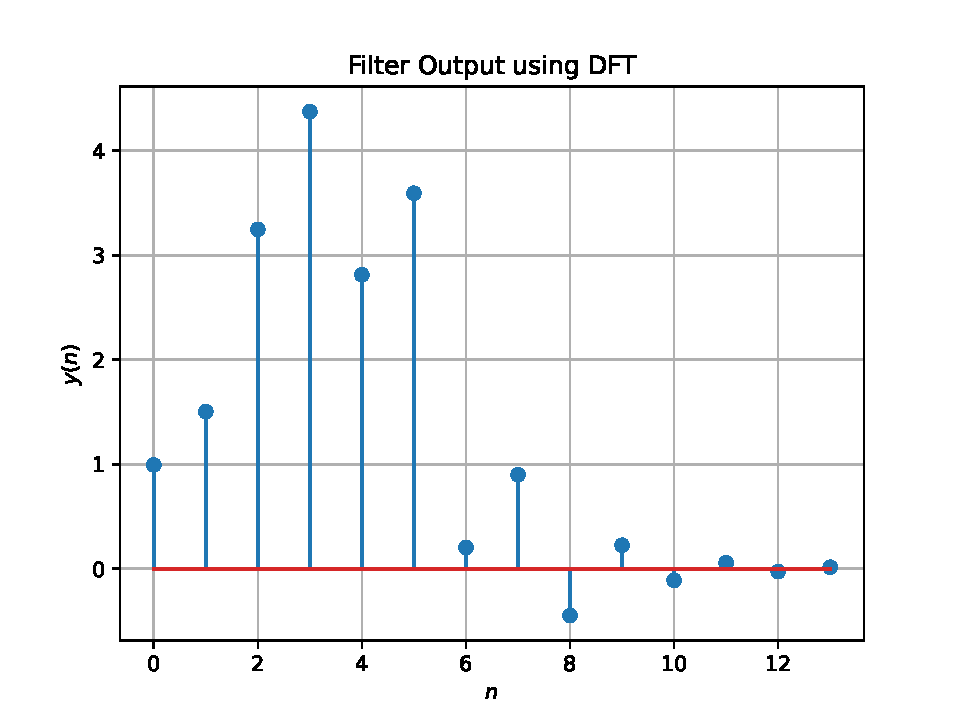
\includegraphics[width=\columnwidth]{figs/prob_6-3.pdf}
		\caption{$y(n)$ from the DFT}
		\label{fig:y-n-dft}
	\end{figure}
	\item Repeat the previous exercise by computing $X(k), H(k)$ and $y(n)$ through FFT and 
	IFFT.
	\solution Download the code from
	\begin{lstlisting}
		$ wget https://raw.githubusercontent.com/prajwal-3-14159/EE3900_ma20btech11013/main/filter/codes/problem_6-4.py
	\end{lstlisting}
	Observe that Fig. \eqref{fig:y-n-fft} is the same as $y(n)$ in Fig. \eqref{fig:xnyn}.
	\begin{figure}
		\centering
		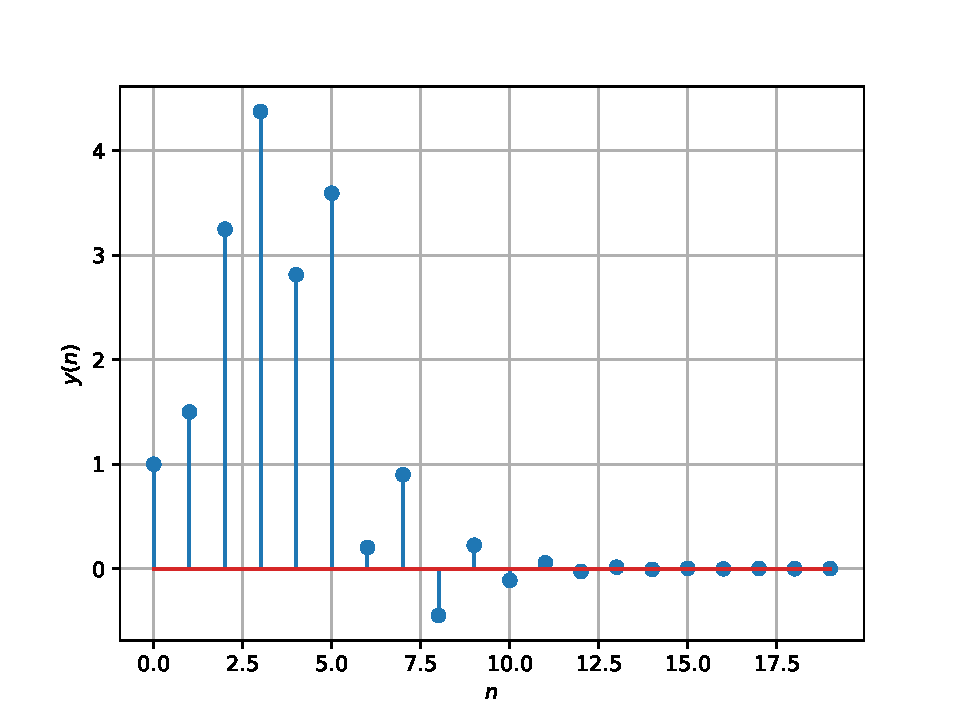
\includegraphics[width=\columnwidth]{figs/prob_6-4.pdf}
		\caption{$y(n)$ using FFT and IFFT}
		\label{fig:y-n-fft}
	\end{figure}
	\begin{figure}[!ht]
		\centering
		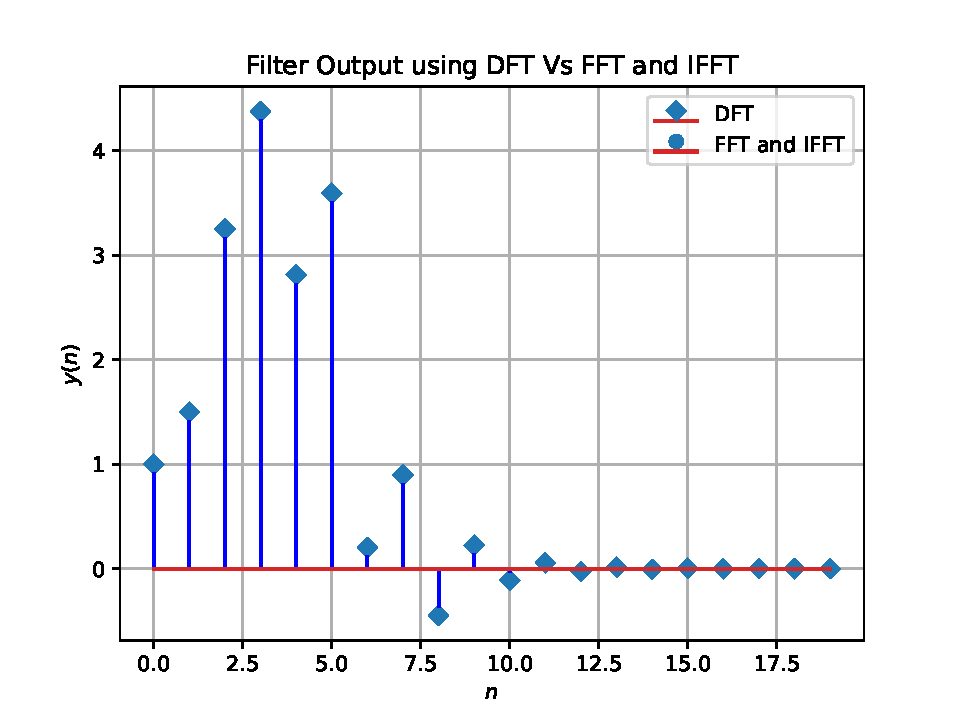
\includegraphics[width=\columnwidth]{figs/prob_6.pdf}
		\caption{$y(n)$ by DFT vs FTT and IFFT}
		\label{fig:y-n-dft_fft}
	\end{figure}
	\item Wherever possible, express all the above equations as matrix equations.
	\solution
	We use the DFT Matrix, where $\omega = e^{-\frac{j2k\pi}{N}}$, which is given by
	\begin{align}
		\mtx{W} = 
		\begin{pmatrix}
			\omega^0 & \omega^0 & \ldots & \omega^0 \\
			\omega^0 & \omega^1 & \ldots & \omega^{N - 1} \\
			\vdots & \vdots & \ddots & \vdots \\
			\omega^0 & \omega^{N - 1} & \ldots & \omega^{(N -1)(N - 1)}
		\end{pmatrix}
	\end{align}
	i.e. $W_{jk} = \omega^{jk}$, $0 \leq j, k < N$. Hence, we can write any DFT equation as
	\begin{align}
		\mtx{X} = \mtx{W}\mtx{x} = \mtx{x}\mtx{W}
	\end{align}
	\noindent where
	\begin{align}
		\mtx{x} = 
		\begin{pmatrix}
			x(0) \\ x(1) \\ \vdots \\ x(n - 1)
		\end{pmatrix}
	\end{align}
	\noindent Using \eqref{eq:inv-ft}, the inverse Fourier Transform is given by
	\begin{align}
		\mtx{x} = \mathcal{F}^{-1}\brak{\mtx{X}} = \mtx{W}^{-1}\mtx{X} &= 
		\frac{1}{N}\mtx{W^{H}}\mtx{X} = \frac{1}{N}\mtx{X}\mtx{W^{H}} \\ 
		\implies \mtx{W}^{-1} &= \frac{1}{N}\mtx{W^{H}}
	\end{align}
	\noindent where $H$ denotes hermitian operator. We can rewrite \eqref{eq:fp} using the
	element-wise multiplication operator as
	\begin{align}
		\mtx{Y} = \mtx{H}\cdot\mtx{X} = \brak{\mtx{W}\mtx{h}}\cdot\brak{\mtx{W}\mtx{x}}
	\end{align}
	The plot of $y(n)$ using the DFT matrix in Fig. \eqref{fig:yn-mtx} is the same as $y(n)$ in 
	Fig. \eqref{fig:xnyn}. Download the code using
	\begin{lstlisting}
		$ wget https://raw.githubusercontent.com/prajwal-3-14159/EE3900_ma20btech11013/main/filter/codes/problem_6-5.py
	\end{lstlisting}
\end{enumerate}
\begin{figure}[!htb]
	\centering
	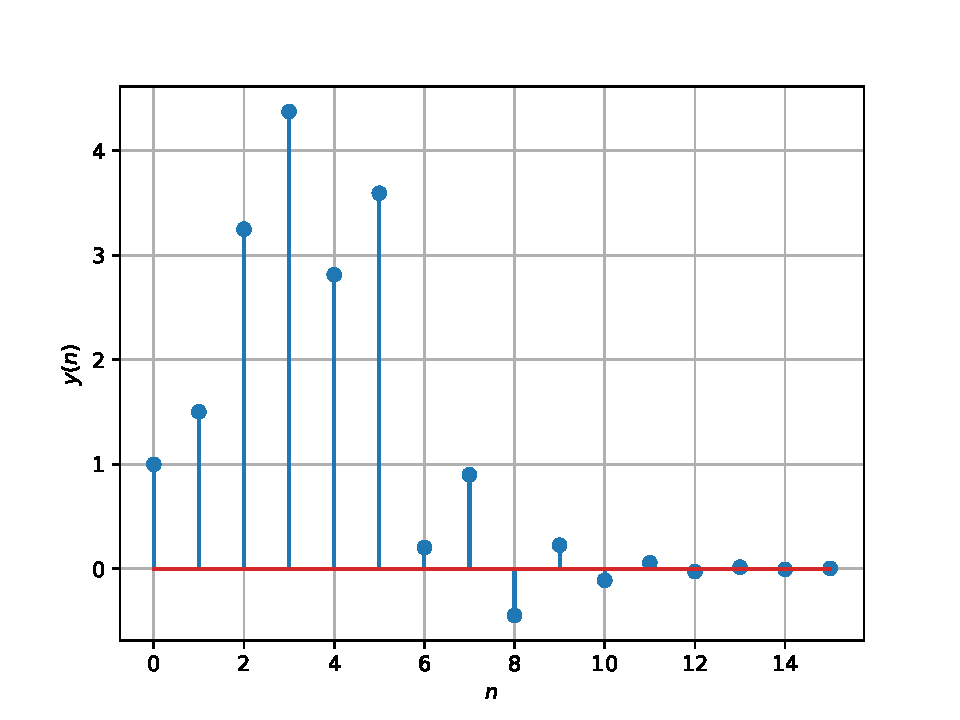
\includegraphics[width=\columnwidth]{figs/prob_6-5.pdf}
	\caption{$y(n)$ using the DFT matrix}
	\label{fig:yn-mtx}
\end{figure}
%\vspace{2cm}
\section{FFT}
% \subsection{Definitions}
\begin{enumerate}[label=\arabic*.,ref=\thesection.\theenumi]
	\numberwithin{equation}{section}
	\item The DFT of $x(n)$ is given by
	\begin{align}
		X(k) \triangleq \sum_{n=0}^{N-1} x(n) e^{-j 2 \pi k n / N}, \quad k=0,1, \ldots, N-1
	\end{align}
	\item Let 
	\begin{align}
		W_{N} = e^{-j2\pi/N} 
	\end{align}
	Then the $N$-point {\em DFT matrix} is defined as 
	\begin{align}
		\vec{F}_{N} = \sbrak{W_{N}^{mn}}, \quad 0 \le m,n \le N-1 
	\end{align}
	where $W_{N}^{mn}$ are the elements of $\vec{F}_{N}$.
	\item Let 
	\begin{align}
		\vec{I}_4 = \myvec{\vec{e}_4^{1} &\vec{e}_4^{2} &\vec{e}_4^{3} &\vec{e}_4^{4} }
	\end{align}
	be the $4\times 4$ identity matrix.  Then the 4 point {\em DFT permutation matrix} is defined as 
	\begin{align}
		\vec{P}_4 = \myvec{\vec{e}_4^{1} &\vec{e}_4^{3} &\vec{e}_4^{2} &\vec{e}_4^{4} }
	\end{align}
	\item The 4 point {\em DFT diagonal matrix} is defined as 
	\begin{align}
		\vec{D}_4 = diag\myvec{W_{4}^{0} & W_{4}^{1} & W_{4}^{2} & W_{4}^{3}}
	\end{align}
	\item Show that 
	\begin{equation}
		W_{N}^{2}=W_{N/2}
	\end{equation}
	\solution\begin{align}
		W_{N} = e^{-j2\pi/N}\\
		\implies W_{N/2} = e^{-j2\pi/(N/2)}\\
		\therefore W_{N}^{2} = e^{2 (-j2\pi/N)} = e^{-j2\pi/(N/2)} = W_{N/2}
	\end{align}
	%    \item Find $\vec{P}_6$.
	%    \item Find $\vec{D}_3$.
	\item Show that 
	\begin{align}
		\vec{F}_{4}=
		\begin{bmatrix}
			\vec{I}_{2} & \vec{D}_{2} \\
			\vec{I}_{2} & -\vec{D}_{2}
		\end{bmatrix}
		\begin{bmatrix}
			\vec{F}_{2} & 0 \\
			0 & \vec{F}_{2}
		\end{bmatrix}
		\vec{P}_{4}
	\end{align}
	\solution
	\begin{align}
		\vec{F}_{2} = 
		\begin{bmatrix}
			W_{2}^0	&	W_{2}^0\\
			W_{2}^0	&	W_{2}^1
		\end{bmatrix}
		=		\begin{bmatrix}
			1	&	1\\
			1	&	-1
		\end{bmatrix}\\
		\vec{D}_{4/2} =
		\begin{bmatrix}
			W_4^0 &	0\\
			0	&	W_4^1 
		\end{bmatrix}
		=\begin{bmatrix}
			1	&	0\\
			0	&	-i 
		\end{bmatrix}\\
		\text{R.H.S } = 
		\begin{bmatrix}
			\vec{F}_{2} & \vec{D}_{4/2} \vec{F}_{2}\\
			\vec{F}_{2} & -\vec{D}_{4/2} \vec{F}_{2}\\
		\end{bmatrix}\vec{P}_{4}\\
		%	=\begin{bmatrix}
			%		W_{2}^0	&	W_{2}^0	&	(W_{2}^0)^2	&	(W_{2}^0)^2\\
			%		W_{2}^0	&	W_{2}^1	&	W_{2}^0 W_{2}^1	&	(W_{2}^1)^2\\
			%		W_{2}^0	&	W_{2}^0	&	-(W_{2}^0)^2	&	-(W_{2}^0)^2\\
			%		W_{2}^0	&	W_{2}^1	&	-W_{2}^0 W_{2}^1	&	-(W_{2}^1)^2\\
			%	\end{bmatrix}\vec{P}_{4}\\
		=\begin{bmatrix}
			1	&	1	&	1	&	1\\
			1	&	-1	&	-i	&	i\\
			1	&	1	&	-1	&	-1\\
			1	&	-1	&	i	&	-i\\
		\end{bmatrix}\vec{P}_{4}\\
		=\begin{bmatrix}
			1	&	1	&	1	&	1\\
			1	&	-i	&	-1	&	i\\
			1	&	-1	&	1	&	-1\\
			1	&	i	&	-1	&	-i\\
		\end{bmatrix}\\
		= \begin{bmatrix}
			W_{4}^0	&	W_{4}^0	&	W_{4}^0	&	W_{4}^0\\
			W_{4}^0	&	W_{4}^1	&	W_{4}^2	&	W_{4}^3\\
			W_{4}^0	&	W_{4}^2	&	W_{4}^4	&	W_{4}^6\\
			W_{4}^0	&	W_{4}^3	&	W_{4}^6	&	W_{4}^9\\
		\end{bmatrix} = \vec{F}_{4}
	\end{align}
	\item Show that 
	\begin{equation}
		\vec{F}_{N}=
		\begin{bmatrix}
			\vec{I}_{N/2} & \vec{D}_{N/2} \\
			\vec{I}_{N/2} & -\vec{D}_{N/2}
		\end{bmatrix}
		\begin{bmatrix}
			\vec{F}_{N/2} & 0 \\
			0 & \vec{F}_{N/2}
		\end{bmatrix}
		\vec{P}_{N}
	\end{equation}
	\item Find 
	\begin{align}
		\vec{P}_4 \vec{x}
	\end{align}
	\solution
	\begin{align}
		\vec{P}_{4} = \myvec{\vec{e}_4^{1} &\vec{e}_4^{3} &\vec{e}_4^{2}	&\vec{e}_4^{4}}\\
		\vec{x}_4 = \myvec{1 & 2 & 3 & 4}\\% & 2 & 1 & \text{\small ignored}\\
		\vec{P}_{4}	\vec{x} = \myvec{1 & 3 & 2 & 4}
	\end{align}
	\item Show that 
	\begin{align}
		\vec{X} = \vec{F}_N \vec{x}
		\label{eq:dft-mat-def}
	\end{align}
	where $\vec{x}, \vec{X}$ are the vector representations of $x(n), X(k)$ respectively.\\
	\solution
	\begin{align}
		\brak{\vec{F}_{N}\vec{x}}_{k} = \sum_{m=0}^{N-1}W_{N}^{mk}x(m)\\
		= \sum_{m=0}^{N-1} x(m) e^{-j 2 \pi k m / N}
		= X(k) = \vec{X}_{k} 
	\end{align}
	\item Derive the following Step-by-step visualisation  of
	8-point FFTs into 4-point FFTs and so on
	\begin{equation}
		\begin{bmatrix}
			X(0) \\ 
			X(1) \\ 
			X(2) \\ 
			X(3)
		\end{bmatrix}
		=
		\begin{bmatrix}
			X_{1}(0) \\ 
			X_{1}(1)\\ 
			X_{1}(2)\\
			X_{1}(3)\\
		\end{bmatrix}
		+
		\begin{bmatrix}
			W^{0}_{8} & 0 & 0 & 0\\
			0 & W^{1}_{8} & 0 & 0\\
			0 & 0 & W^{2}_{8} & 0\\
			0 & 0 & 0 & W^{3}_{8}
		\end{bmatrix}
		\begin{bmatrix}
			X_{2}(0) \\ 
			X_{2}(1) \\ 
			X_{2}(2) \\
			X_{2}(3)
		\end{bmatrix}
	\end{equation}
	\begin{equation}
		\begin{bmatrix}
			X(4) \\ 
			X(5) \\ 
			X(6) \\ 
			X(7)
		\end{bmatrix}
		=
		\begin{bmatrix}
			X_{1}(0) \\ 
			X_{1}(1)\\ 
			X_{1}(2)\\
			X_{1}(3)\\
		\end{bmatrix}
		-
		\begin{bmatrix}
			W^{0}_{8} & 0 & 0 & 0\\
			0 & W^{1}_{8} & 0 & 0\\
			0 & 0 & W^{2}_{8} & 0\\
			0 & 0 & 0 & W^{3}_{8}
		\end{bmatrix}
		\begin{bmatrix}
			X_{2}(0) \\ 
			X_{2}(1) \\ 
			X_{2}(2) \\
			X_{2}(3)
		\end{bmatrix}
	\end{equation}
	4-point FFTs into 2-point FFTs
	\begin{equation}
		\begin{bmatrix}
			X_{1}(0) \\ 
			X_{1}(1)\\ 
		\end{bmatrix}
		=
		\begin{bmatrix}
			X_{3}(0) \\ 
			X_{3}(1)\\ 
		\end{bmatrix}
		+
		\begin{bmatrix}
			W^{0}_{4} & 0\\
			0 & W^{1}_{4}
		\end{bmatrix}
		\begin{bmatrix}
			X_{4}(0) \\ 
			X_{4}(1) \\ 
		\end{bmatrix}
	\end{equation}
	\begin{equation}
		\begin{bmatrix}
			X_{1}(2) \\ 
			X_{1}(3)\\ 
		\end{bmatrix}
		=
		\begin{bmatrix}
			X_{3}(0) \\ 
			X_{3}(1)\\ 
		\end{bmatrix}
		-
		\begin{bmatrix}
			W^{0}_{4} & 0\\
			0 & W^{1}_{4}
		\end{bmatrix}
		\begin{bmatrix}
			X_{4}(0) \\ 
			X_{4}(1) \\ 
		\end{bmatrix}
	\end{equation}
	\begin{equation}
		\begin{bmatrix}
			X_{2}(0) \\ 
			X_{2}(1)\\ 
		\end{bmatrix}
		=
		\begin{bmatrix}
			X_{5}(0) \\ 
			X_{5}(1)\\ 
		\end{bmatrix}
		+
		\begin{bmatrix}
			W^{0}_{4} & 0\\
			0 & W^{1}_{4}
		\end{bmatrix}
		\begin{bmatrix}
			X_{6}(0) \\ 
			X_{6}(1) \\ 
		\end{bmatrix}
	\end{equation}
	\begin{equation}
		\begin{bmatrix}
			X_{2}(2) \\ 
			X_{2}(3)\\ 
		\end{bmatrix}
		=
		\begin{bmatrix}
			X_{5}(0) \\ 
			X_{5}(1)\\ 
		\end{bmatrix}
		-
		\begin{bmatrix}
			W^{0}_{4} & 0\\
			0 & W^{1}_{4}
		\end{bmatrix}
		\begin{bmatrix}
			X_{6}(0) \\ 
			X_{6}(1) \\ 
		\end{bmatrix}
	\end{equation}
	\begin{equation}
		P_{8}
		\begin{bmatrix}
			x(0) \\ 
			x(1) \\ 
			x(2) \\ 
			x(3) \\ 
			x(4) \\ 
			x(5) \\
			x(6) \\
			x(7)
		\end{bmatrix}
		= 
		\begin{bmatrix}
			x(0) \\ 
			x(2) \\ 
			x(4) \\ 
			x(6) \\
			x(1) \\ 
			x(3) \\ 
			x(5) \\
			x(7)
		\end{bmatrix}
	\end{equation}
	\begin{equation}
		P_{4}
		\begin{bmatrix}
			x(0) \\ 
			x(2) \\ 
			x(4) \\ 
			x(6) \\
		\end{bmatrix}
		= 
		\begin{bmatrix}
			x(0) \\ 
			x(4) \\ 
			x(2) \\
			x(6)
		\end{bmatrix}
	\end{equation}
	\begin{equation}
		P_{4}
		\begin{bmatrix}
			x(1) \\ 
			x(3) \\ 
			x(5) \\
			x(7)
		\end{bmatrix}
		= 
		\begin{bmatrix}
			x(1) \\ 
			x(5) \\ 
			x(3) \\ 
			x(7) \\
		\end{bmatrix}
	\end{equation}
	Therefore,
	\begin{equation}
		\begin{bmatrix}
			X_{3}(0) \\ 
			X_{3}(1)\\ 
		\end{bmatrix}
		= F_{2}
		\begin{bmatrix}
			x(0) \\ 
			x(4) \\ 
		\end{bmatrix}
	\end{equation}
	\begin{equation}
		\begin{bmatrix}
			X_{4}(0) \\ 
			X_{4}(1)\\ 
		\end{bmatrix}
		= F_{2}
		\begin{bmatrix}
			x(2) \\ 
			x(6) \\ 
		\end{bmatrix}
	\end{equation}
	\begin{equation}
		\begin{bmatrix}
			X_{5}(0) \\ 
			X_{5}(1)\\ 
		\end{bmatrix}
		= F_{2}
		\begin{bmatrix}
			x(1) \\ 
			x(5) \\ 
		\end{bmatrix}
	\end{equation}
	\begin{equation}
		\begin{bmatrix}
			X_{6}(0) \\ 
			X_{6}(1)\\ 
		\end{bmatrix}
		= F_{2}
		\begin{bmatrix}
			x(3) \\ 
			x(7) \\ 
		\end{bmatrix}
	\end{equation}
	\item For 
	\begin{align}
		\vec{x} = \myvec{1\\2\\3\\4\\2\\1}
		\label{eq:equation1}
	\end{align}
	compte the DFT  
	using 
	\eqref{eq:dft-mat-def}\\
	\solution
	\begin{align}
		\vec{X} = \vec{F}_6 \vec{x}
	\end{align}	
	\begin{align}
		= \begin{bsmallmatrix}
			1	&	1	&	1	&	1	&	1	&	1\\
			1	&	\brak{e^{\frac{-j2\pi}{6}}}	&	\brak{e^{\frac{-j2\pi}{6}}}^2	&	\brak{e^{\frac{-j2\pi}{6}}}^3	&	\brak{e^{\frac{-j2\pi}{6}}}^4	&	\brak{e^{\frac{-j2\pi}{6}}}^5\\
			1	&	\brak{e^{\frac{-j2\pi}{6}}}^2	&	\brak{e^{\frac{-j2\pi}{6}}}^4	&	\brak{e^{\frac{-j2\pi}{6}}}^6	&	\brak{e^{\frac{-j2\pi}{6}}}^8	&	\brak{e^{\frac{-j2\pi}{6}}}^{10}\\
			1	&	\brak{e^{\frac{-j2\pi}{6}}}^3	&	\brak{e^{\frac{-j2\pi}{6}}}^6	&	\brak{e^{\frac{-j2\pi}{6}}}^9	&	\brak{e^{\frac{-j2\pi}{6}}}^{12}	&	\brak{e^{\frac{-j2\pi}{6}}}^{15}\\
			1	&	\brak{e^{\frac{-j2\pi}{6}}}^4	&	\brak{e^{\frac{-j2\pi}{6}}}^8	&	\brak{e^{\frac{-j2\pi}{6}}}^{12}	&	\brak{e^{\frac{-j2\pi}{6}}}^{16}	&	\brak{e^{\frac{-j2\pi}{6}}}^{20}\\
			1	&	\brak{e^{\frac{-j2\pi}{6}}}^5	&	\brak{e^{\frac{-j2\pi}{6}}}^{10}	&	\brak{e^{\frac{-j2\pi}{6}}}^{15}	&	\brak{e^{\frac{-j2\pi}{6}}}^{20}	&	\brak{e^{\frac{-j2\pi}{6}}}^{25}
		\end{bsmallmatrix}
		\myvec{1\\2\\3\\4\\2\\1}
	\end{align}
	\begin{align}
		=\myvec{13\\-4 - \sqrt{3}j\\ 1\\-1\\1\\-4 + \sqrt{3}j}
	\end{align}
	\item Repeat the above exercise using the FFT
	after zero padding $\vec{x}$.\\
	\solution
	\begin{lstlisting}
		wget https://github.com/DarkWake9/EE3900/blob/main/Assignment%201/e7.12.py
	\end{lstlisting}
	From the above code we get this output:
	$\begin{bmatrix}
		13\\
		-3.1213-6.5355j\\
		j\\
		1.1213-0.5355j\\
		-1\\
		1.1213+0.5355j\\
		-j\\
		-3.1213+6.5355j
	\end{bmatrix}$
	%	    \eqref{eq:fft-mat-def}
	\item Write a C program to compute the 8-point FFT. \\
	\solution
	\begin{lstlisting}
		wget https://github.com/DarkWake9/EE3900/blob/main/Assignment%201/e7.13.c
	\end{lstlisting}
	From the above code we get this output:
	$\begin{bmatrix}
		13\\
		-3.1327 - j6.5545\\
		j\\
		1.1327 - j0.5545\\
		-1\\
		1.1327 + j0.5545\\
		- j\\
		-3.1327 + j6.5545\\
	\end{bmatrix}$
	\vspace{1cm}
\end{enumerate}

\section{Exercises}
\noindent Answer the following questions by looking at the python code in Problem \ref{prob:output}.
\begin{enumerate}[label=\thesection.\arabic*]
	\item
	The command
	\begin{lstlisting}
		output_signal = signal.lfilter(b, a, input_signal)
	\end{lstlisting}
	in Problem \ref{prob:output} is executed through the following difference equation
	\begin{equation}
		\label{eq:iir_filter_gen}
		\sum _{m=0}^{M}a\brak{m}y\brak{n-m}=\sum _{k=0}^{N}b\brak{k}x\brak{n-k}
	\end{equation}
	where the input signal is $x(n)$ and the output signal is $y(n)$ with initial values all 0. Replace
	\textbf{signal.filtfilt} with your own routine and verify.
	\solution
	The implementation is at
	\begin{lstlisting}
		$ wget https://raw.githubusercontent.com/prajwal-3-14159/EE3900_ma20btech11013/main/filter/codes/problem_7-1.py
	\end{lstlisting}
	\item Repeat all the exercises in the previous sections for the above $a$ and $b$.
	\solution
	%\begin{align}
	%	\mtx{a} =
	%	\begin{pmatrix}
		%		4.44 \\ 8.78 \\ -9.93 \\ 6.90 \\ -2.93 \\ 0.70 \\ -0.07
		%	\end{pmatrix}
	%	\mtx{b} = 
	%	\begin{pmatrix}
		%		5.02 \times 10^{-5} \\ 3.52 \times 10^{-4} \\ 1.05 \times 10^{-3} \\ 1.76 \times 10^{-3} \\ 1.76 \times 10^{-3} \\ 1.05 \times 10^{-3} \\ 3.52 \times 10^{-4} \\ 5.02 \times 10^{-5} 
		%	\end{pmatrix}
	%\end{align}
	For the given values, the difference equation is
	\begin{align}
		&y(n) - \brak{4.44}y(n - 1) + \brak{8.78}y(n - 2) \nonumber \\
		&- \brak{9.93}y(n - 3) + \brak{6.90}y(n - 4) \nonumber \\
		&- \brak{2.93}y(n - 5) \nonumber + \brak{0.70}y(n - 6) \nonumber \\
		&- \brak{0.07}y(n - 7) = \brak{5.02 \times 10^{-5}}x(n) \nonumber \\
		&+ \brak{3.52 \times 10^{-4}}x(n - 1) + \brak{1.05 \times 10^{-3}}x(n - 2) \nonumber \\
		&+ \brak{1.76 \times 10^{-3}}x(n - 3) + \brak{1.76 \times 10^{-3}}x(n - 4) \nonumber \\
		&+ \brak{1.05 \times 10^{-3}}x(n - 5) + \brak{3.52 \times 10^{-4}}x(n - 6) \nonumber \\
		&+ \brak{5.02 \times 10^{-5}}x(n - 7)
	\end{align}
	From \eqref{eq:iir_filter_gen}, we see that the transfer function can be written as follows
	\begin{align}
		H(z) &= \frac{\sum_{k = 0}^{N}b(k)z^{-k}}{\sum_{k = 0}^{M}a(k)z^{-k}} \\
		&= \sum_{i}\frac{r(i)}{1 - p(i)z^{-1}} + \sum_{j}k(j)z^{-j}
		\label{eq:trans-func}
	\end{align}
	where $r(i)$, $p(i)$, are called residues and poles respectively of the partial 
	fraction expansion of $H(z)$. $k(i)$ are the coefficients of the direct polynomial 
	terms that might be left over. We can now take the inverse $z$-transform of
	\eqref{eq:trans-func} and get using \eqref{eq:anun},
	\begin{align}
		h(n) &= \sum_{i}r(i)[p(i)]^nu(n) + \sum_{j}k(j)\delta(n - j)
		\label{eq:h-n-expr}
	\end{align}
	Substituting the values,
	\begin{align}
		&h(n) = [\brak{2.76}\brak{0.55}^n \nonumber \\ 
		&+ \brak{-1.05-1.84\j}\brak{0.57+0.16\j}^n \nonumber \\
		&+ \brak{-1.05+1.84\j}\brak{0.57-0.16\j}^n \nonumber \\
		&+ \brak{-0.53+0.08\j}\brak{0.63+0.32\j}^n \nonumber \\
		&+ \brak{-0.53-0.08\j}\brak{0.63-0.32\j}^n \nonumber \\
		&+ \brak{0.20+0.004\j}\brak{0.75+0.47\j}^n \nonumber \\
		&+ \brak{0.20-0.004\j}\brak{0.75-0.47\j}^n]u(n) \nonumber \\
		&+ \brak{-6.81 \times 10^{-4}}\delta(n)
	\end{align}
	The values $r(i)$, $p(i)$, $k(i)$ and thus the impulse response function are computed and plotted at
	\begin{lstlisting}
		$ wget https://raw.githubusercontent.com/prajwal-3-14159/EE3900_ma20btech11013/main/filter/codes/problem_7-2-1.py
	\end{lstlisting}
	The filter frequency response is plotted at
	\begin{lstlisting}
		$ wget https://raw.githubusercontent.com/prajwal-3-14159/EE3900_ma20btech11013/main/filter/codes/problem_7-2-2.py
	\end{lstlisting}
	Observe that for a series $t_n = r^n$, $\frac{t_{n + 1}}{t_n} = r$.
	By the ratio test, $t_n$ converges if $|r| < 1$. We note that
	observe that $|p(i)| < 1$ and so, as $h(n)$ is the sum of convergent series,
	we see that $h(n)$ converges. From Fig. \eqref{fig:butter-imp}, it is clear
	that $h(n)$ is bounded. From \eqref{eq:z_trans},
	\begin{align}
		\sum_{n = 0}^{\infty}h(n) = H(1) = 1 < \infty
	\end{align}
	Therefore, the system is stable. From
	Fig. \eqref{fig:butter-imp}, $h(n)$ is negligible after $n \geq 64$, and we
	can apply a 64-bit FFT to get y(n). The following code uses the DFT matrix
	to generate $y(n)$ in Fig. \eqref{fig:butter-out}.
	\begin{lstlisting}
		$ wget https://raw.githubusercontent.com/prajwal-3-14159/EE3900_ma20btech11013/main/filter/codes/problem_7-2-3.py
	\end{lstlisting}
	\begin{figure}[!htb]
		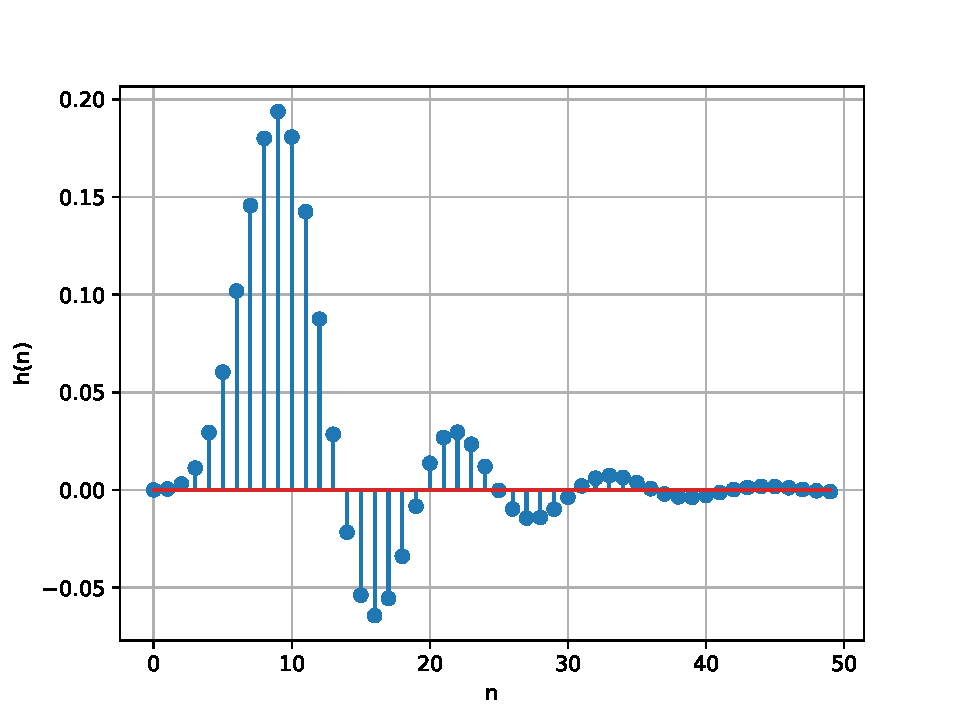
\includegraphics[width=\columnwidth]{figs/prob_7-2-1.pdf}
		\caption{Plot of $h(n)$}
		\label{fig:butter-imp}
	\end{figure}
	\begin{figure}[!htb]
		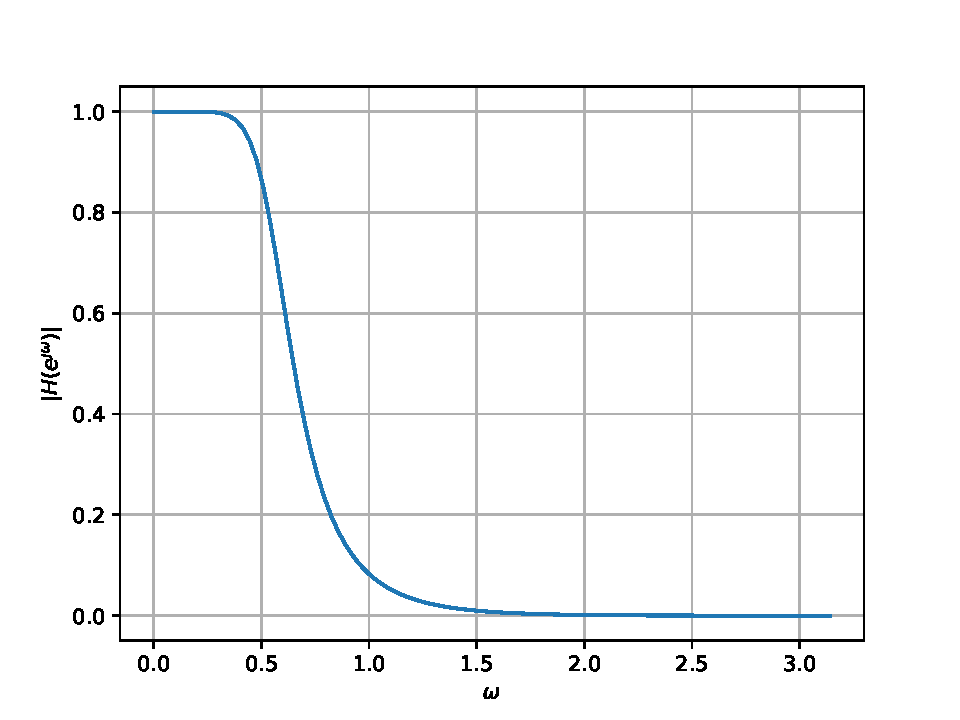
\includegraphics[width=\columnwidth]{figs/prob_7-2-2.pdf}
		\caption{Filter frequency response}
		\label{fig:butter-resp}
	\end{figure}
	\begin{figure}[!htb]
		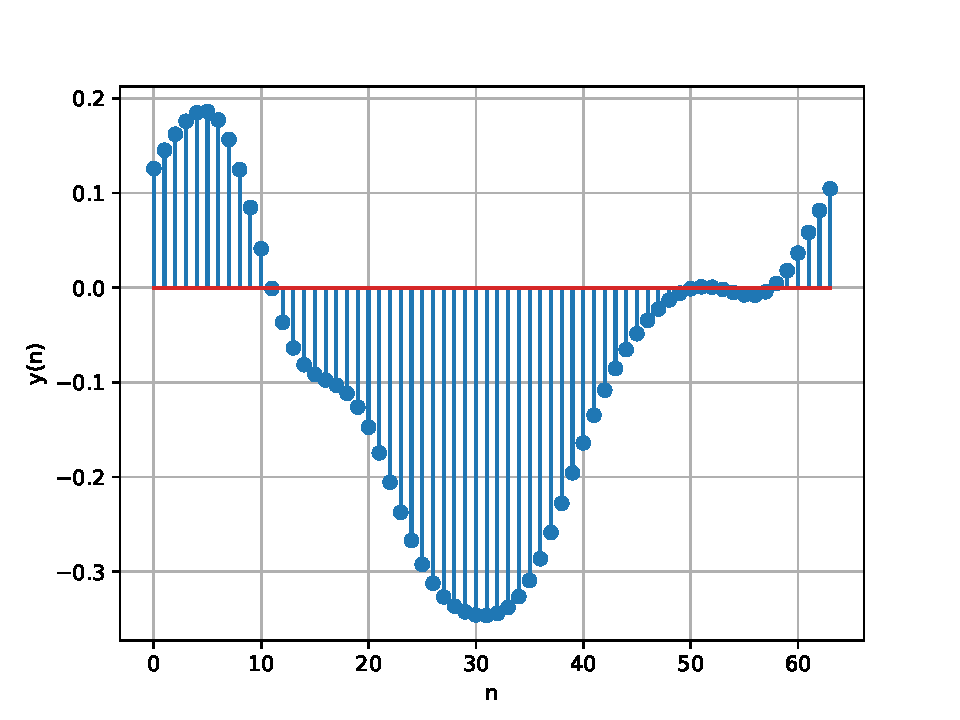
\includegraphics[width=\columnwidth]{figs/prob_7-2-3.pdf}
		\caption{Plot of $y(n)$}
		\label{fig:butter-out}
	\end{figure}
	\item What is the sampling frequency of the input signal?
	\solution
	Sampling frequency $f_s = 44.1$ kHZ.
	\item
	What is type, order and  cutoff frequency of the above Butterworth filter?
	\solution
	The given Butterworth filter is low pass with order 4 and cutoff frequency 4 kHz.
	\item
	Modifying the code with different input parameters and to get the best possible output.
	\solution
	A better filtering was found on setting the order of the filter to be 7.
\end{enumerate}
\end{document}